\chapter{Introducción}

\section{Consideraciones iniciales}

\subsection{Definición}

Scrum es un marco de trabajo (framework) para construir y mantener productos complejos \cite{SBOK-2013} \cite{Scrum-Alliance-2015}. 
Scrum funciona como una implementación del ciclo de mejora continua de Deming (PDCA) y como una implementación de los principios ágiles y principios Scrum. Hay que tener en cuenta que Scrum no es exactamente un proceso íntegro, metodología completa o una técnica para construir productos; sino que, es un marco de trabajo dentro del cual se pueden emplear varias técnicas y procesos \cite{Agile-Atlas-2012}. 

\subsection{Sobre si es una Metodología}

Hay quienes consideran que Scrum no es una metodología, entre otras cosas porque no especifia exactamente el cómo se hacen las cosas, 
sino que dice el qué hacer. Sin embrargo, hay autores y guías que tratan a Scrum como metodología \cite{SBOK-2013}. De hecho en el informe original de Ken Schwaber se habla de metodología \cite{Ken-Schwaber-1995}. En consecuencia, se puede encontrar en numerosa bibliografía que el marco de trabajo Scrum puede ser denominado "Metodología de Desarrollo Scrum" o "Metodología de Gestión de Proyectos Scrum". 
En el primer caso puede deberse a que se puede considerar una metodología como un proceso de desarrollo iterativo e incremental de productos \cite{Ken-Schwaber-1995}. Y en el segundo caso porque se puede considerar que es una alternativa a la gestión clásica de proyectos propuesta por metodologías como la Metodología de Gestión de Proyectos PMI. En este último sentido podemos recordar la definición original de Ken Schwaber: "Scrum es una metodología de gestión, mejora y mantenimiento de un sistema existente o prototipo de producción" \cite{Ken-Schwaber-1995}.
 
Por otro lado, considerando que Scrum define roles, artefactos, actividades, flujo del ciclo de actividades Scrum \cite{Agile-Atlas-2012}, reglas y algunas sugerencias de implementación como, además, al definir el flujo del ciclo de Scrum o flujo de trabajo define parcialmente un cómo, en el cual incluye una secuencia básica de cosas a hacer; por eso, y sin ser puristas, se puede considerar como una forma de metodología de trabajo y de gestión. O sea que puede funcionar como una metodología a alto nivel o plataforma de trabajo sobre la cual pueden funcionar otras metodologías, más específicas de producción y desarrollo, y otras técnicas y procesos. Por este motivo, 
Scrum puede ser adaptado a diversas empresas y organizaciones que trabajen con metodologías diversas pero compatibles con los 
lineamientos de Scrum (sus valores y principios) y del Movimiento Ágil (filosofía ágil). Se puede usar Scrum y a su vez utilizar técnicas de otras metodologías para implementar sus actividades y sugerencias. O sea que cuando se usa Scrum se hace una aproximación empleando diversas técnicas y, posiblemente, otras metodologías.

\subsection{Ámbito de aplicación}

Relacionado a su ámbito de aplicación se pude decir que Scrum no es un marco de trabajo orientado a implementarse en cualquier dominio y contexto. Scrum está pensado para proyectos bajo "dominios complejos" [Snowden 2007] donde existe un grado alto de incertidumbre y baja predictibilidad (ver figura \ref{fig:MarcoCynefinModel}). O sea que es útil en ámbitos con requisitos inciertos y riesgos técnicos altos. Nos permite encontrar prácticas emergentes en dominios complejos, como por ejemplo en la gestión de proyectos de innovación \cite{Martin-Alaimo-2014}. Está orientado a contextos que necesitan niveles altos de creatividad, innovación, interaccion y comunicación. Por este motivo, es bastante empleado en la industria de software, ya que en la misma existen contextos específicos de alta complejidad e incertidumbre con necesidad de creatividad e innovación. Pero también se utiliza en otras industrias con dominios de problemas de complejidad semejante. Por ejemplo ha sido empleado en: educación, organizaciones de campañas publicitarias, industria de productos de innovación, empresas de editoriales de libros, etcétera.

\begin{figure}[h]
  \centering
  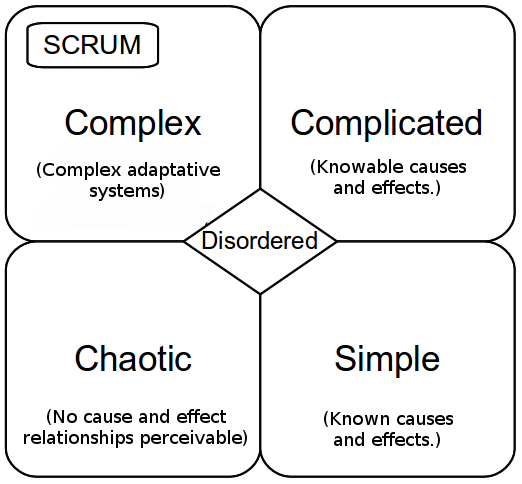
\includegraphics[width=0.50\textwidth]{MarcoCynefinModel}
  \caption{Modelo de dominios de Marco Cynefin}
  \centering
  \label{fig:MarcoCynefinModel} %\ref{fig:MarcoCynefinModel}
\end{figure}

\subsection{Visión general}

En esta metodología se definen los principios y valores a seguir, los roles, relaciones y respnsabilidades, los artefactos o entidades manejadas en el proceso de trabajo, un conjunto de reuniones o actividades en un flujo de trabajo como resume la imagen de la figura \ref{fig:ScrumMapMind}.

\begin{figure}[h]
  \centering
  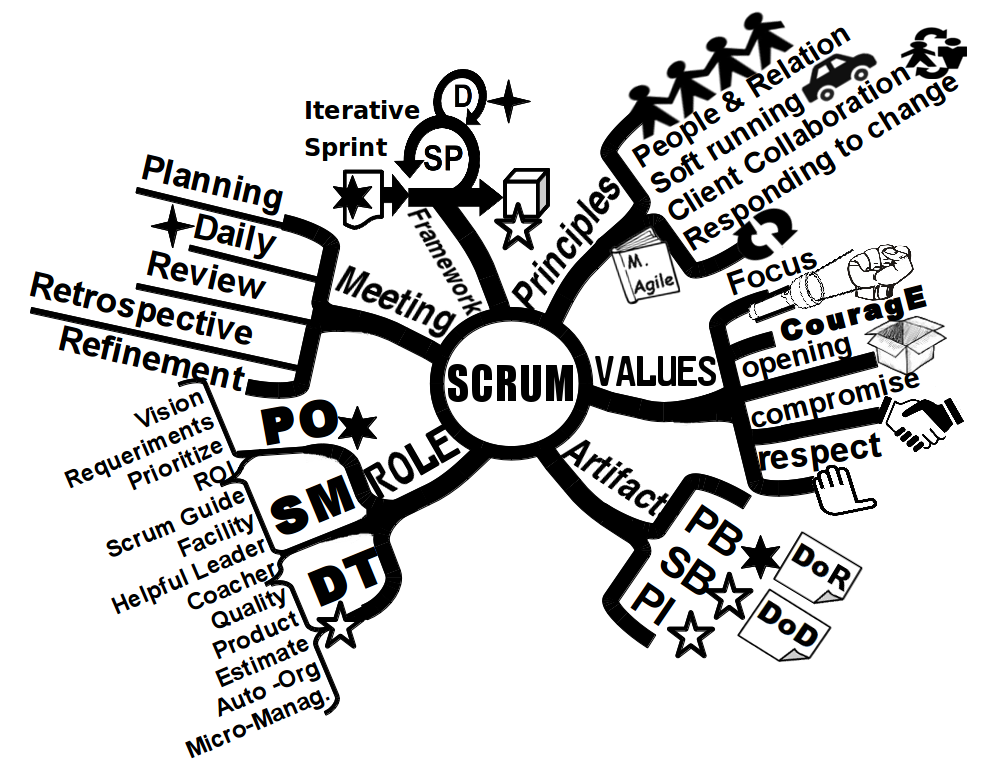
\includegraphics[width=0.99\textwidth]{ScrumMapMind}
  \caption{Mapa mental sobre Scrum}
  \centering
  \label{fig:ScrumMapMind} %\ref{fig:ScrumMapMind}
\end{figure}

En los siguientes capítulos se explicarán los diferentes aspectos y características de la propuesta de este marco de trabajo con lo que 
al final del libro el mapa mental de la figura \ref{fig:ScrumMapMind} quedará explicado y será fácilmente entendible. 
